
\documentclass[12 pt, a4paper]{report}
\usepackage{pdfpages}
\usepackage{graphicx}
\begin{document}
	
	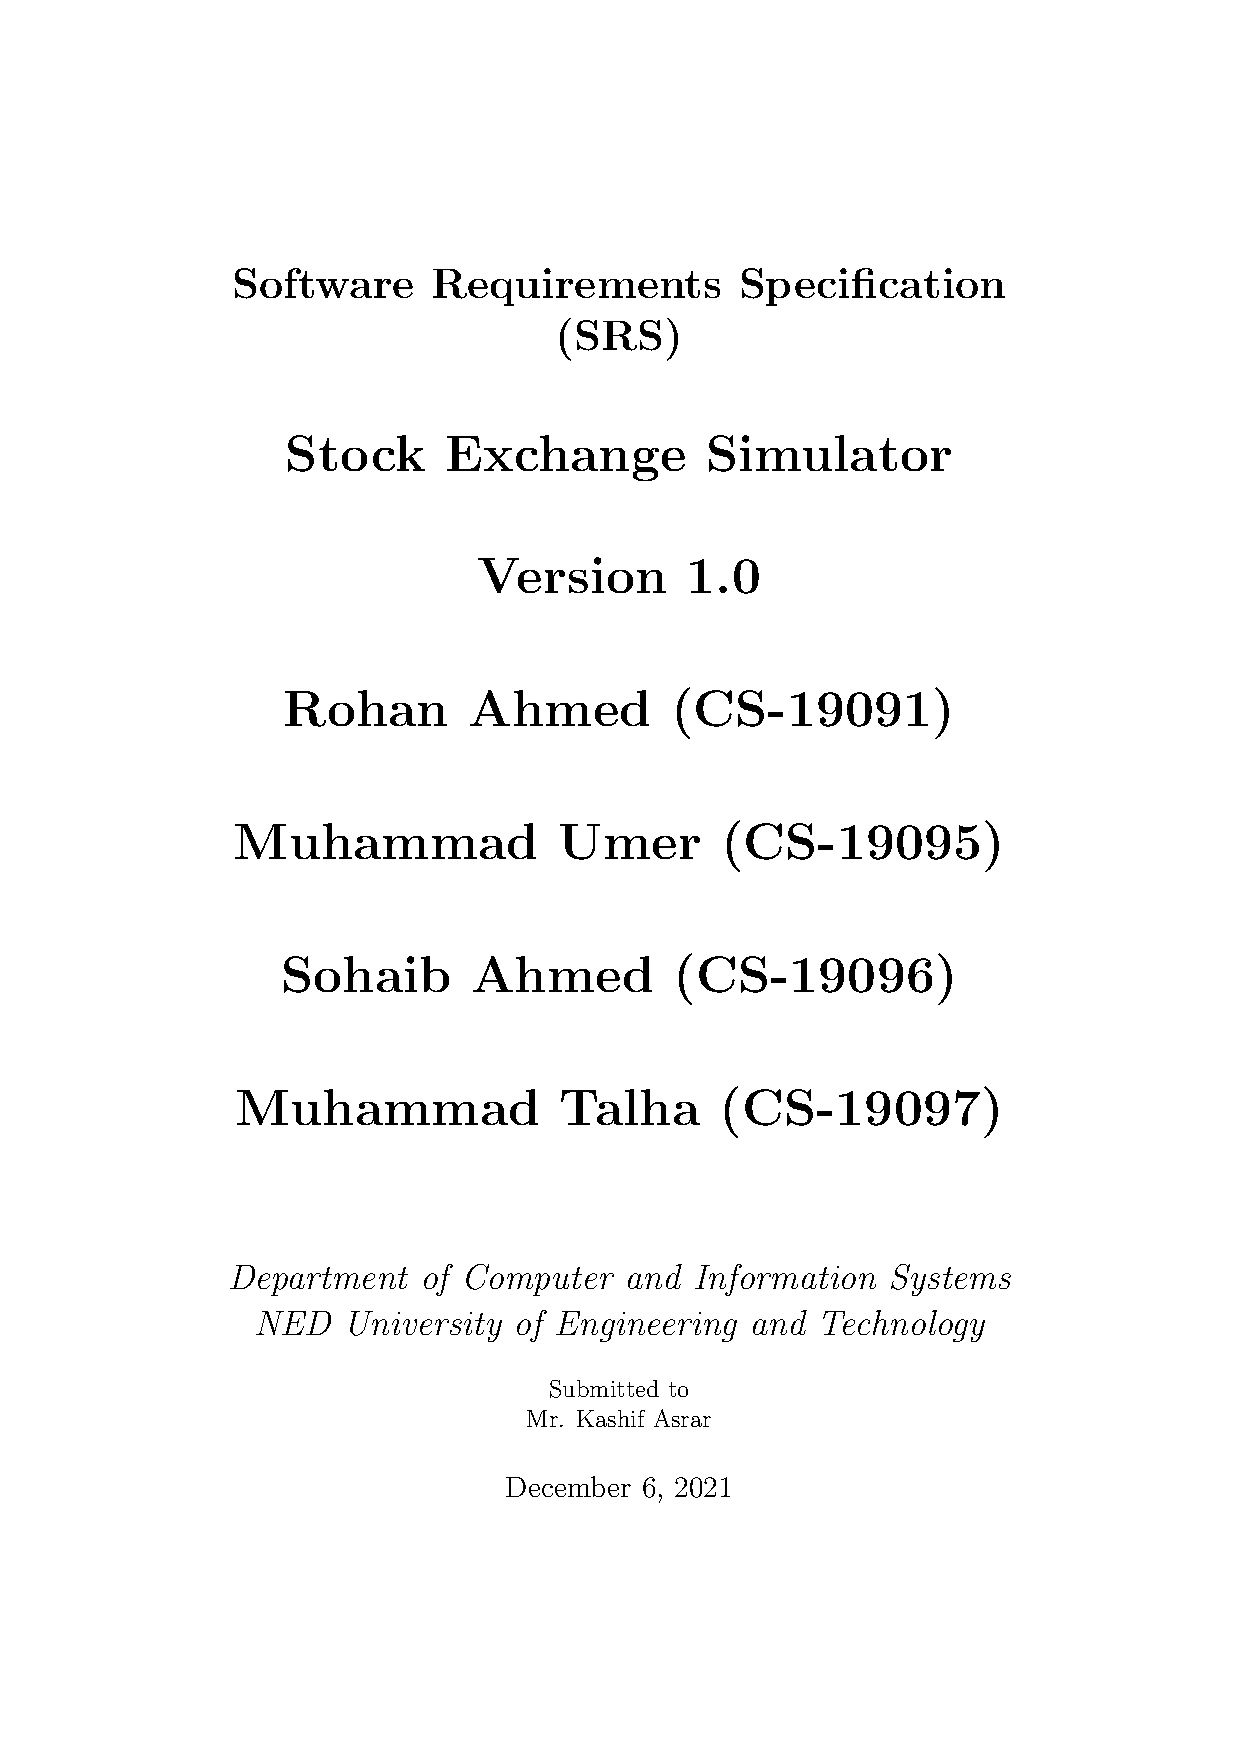
\includepdf{TitlePage}
	\tableofcontents
	\chapter{Introduction}
	
	Stock Exchange Simulator is a desktop application for simulating a real stock exchange. It will allow its users to "buy" and "sell" stocks at real time prices. This section gives an overview of the project and this SRS document.
	\section {Document Purpose}
	The purpose of this SRS is to fully specify all the requirements of the first release of Stock Exchange Simulator (version 1.0) for all stake-holders. The document covers software requirements, hardware requirements, user-interface descriptions, program flows, functional requirements and non-functional requirements.
	
	\section{Product Scope}
	\textit{Provide a short description of the software being specified an its purpose, including relevant benefits, objectives, and goals. TO DO: 1-2 paragraphs describing the scope of the product. Make sure to describe the benefits associated with the product.}
		
	This intention of this project is to simulate a stock exchange environment for  users to learn the basics of stock exchange. This learning process would be simple, stress free, and enjoyable in a gaming environment. This environment allows players to hone their skills through competition with other players using virtual money to  buy and sell stocks based on real stock market data. Through experience, players will gain confidence in their investing abilities. We hope to make the difficult task of learning to invest in a high risk, stock exchange market as an enjoyable experience.
	
	\section{Intended Audience and Document overview}
	\textit{Describe the different types of reader that the document is intended for, such as developers, project managers, marketing staff, users, testers, and documentation writers (In your case it would probably be the “client” and the professor). Describe what the rest of this SRS contains and how it is organized. Suggest a sequence for reading the document, beginning with the overview sections and proceeding through the sections that are most pertinent to each reader type.}
	
	This SRS is intended for the following audiences:
	\begin{itemize}
		\item \textbf{Main Development Team}: The development team will be writing, testing, and deploying the code. The document aims to detailed and unambiguous in its description about the project for the ease of development.
		\item \textbf{Other Developers}: As this project is going to be open source and anyone can contribute to its code, this document also serves purpose of explaining the requirements of the project to developers other than the ones in the main development team so that they can understand the project's functionalities and contribute easily.
		\item \textbf{End Users}: The end users of this application are the people for whom this application is intended for and who will use this application for learning about stock exchange and improve their stock trading skills. The document can be read by the end users to gain in depth insight on how this application works
	\end{itemize}

	\section {Definitions, Acronyms and Abbreviations}
		\textit{Define all the terms necessary to properly interpret the SRS, including acronyms and abbreviations. You may wish to build a separate glossary that spans multiple projects or the entire organization, and just include terms specific to a single project in each SRS. TO DO: Please provide a list of all abbreviations and acronyms used in this document sorted in alphabetical order.}
	\begin{itemize}
		\item \textbf{Framework / Library (in context of programming languages):} Collection of code that perform some often-required functionality, that can be used by anone.
		\item \textbf{Firebase:} A platform/service developed by Google for creating mobile and web applications. Includes various services and features like authentication, database, analytics, and more.
		\item \textbf{Firestore:} A cloud database service included in Firebase
		\item \textbf{SRS:} \textbf{S}oftware \textbf{R}equirements \textbf{S}pecification
		\item \textbf{HTML}: \textbf{H}yper  \textbf{T}ext \textbf{M}arkup \textbf{L}anguage - A language for making structure of user-interfaces
		\item \textbf{CSS:} \textbf{C}ascading \textbf{S}tyle \textbf{S}heets - A language for styling user-interfaces made with HTML.
		\item \textbf{JavaScript (JS for short)}: A programming language, for including logic, interactivity, etc.
		\item \textbf{Node JS}: A JavaScript tool to execute JavaScript outside web-browsers.
		\item \textbf{Electron JS}: A JavaScript tool to make desktop applications.
		\item \textbf{API}: \textbf{A}pplication \textbf{P}rogramming \textbf{I}terface - A software intermediary that allows two applications to talk to each other. (for example our application will communicate with Alpha Vantage API to get stocks related information)
		
	\end{itemize}
	
	
	\section {Document Conventions}
	This document is made using LaTeX, a software system for document prepration. It uses Arial font size 12 pt and 1” margins.
	
	\section {References and Acknowledgments}
	\begin{itemize}
		\item Alpha Vantage API - https://www.alphavantage.co/
		\item Firebase - https://firebase.google.com/
	\end{itemize}
	
	\chapter {Overall Description}
	\section {Product Perspective}
	\textit{Describe the context and origin of the product being specified in this SRS. For example, state whether this product is a follow-on member of a product family, a replacement for certain existing systems, or a new, self-contained product. If the SRS defines a component of a larger system, relate the requirements of the larger system to the functionality of this software and identify interfaces between the two. In this part, make sure to include a simple diagram that shows the major components of the overall system, subsystem interconnections, and external interface. In this section it is crucial that you will be creative and provide as much information as possible. TO DO: Provide at least one paragraph describing product perspective. Provide a general diagram that will illustrate how your product interacts with the environment and in what context it is being used.}\\
	Stock Exchange Simulator is an application for users to learn about stock exchanging without risking real money. This document covers the requirements for the first version (Version 1.0) of the application.
	
	\section {Product Functionality} 
	\textit{Summarize the major functions the product must perform or must let the user perform. Details will be provided in Section 3, so only a high level summary is needed here. Organize the functions to make them understandable to any reader of the SRS. A picture of the major groups of related requirements and how they relate, such as a top level data flow diagram or object class diagram, will be effective.
	TO DO: 
	1. Provide a bulleted list of all the major functions of the system
	2. (Optional) Provide a Data Flow Diagram of the system to show how these functions relate to each other.}

	Following are the major functionalities of this project:
	\begin{itemize}
		\item Users will be able to sign up for a new account.
		\item Users will be able to sign in using an existing account.
		\item Users will be able to view their portfolio including all their stock holdings (and details therof) and cash.
		\item Users will be able to view details of the stocks they have selected to be tracked.
		\item Users will be able to see history of their trading.
		\item Users will be able to find out price of any stock by inputting the stock's symbol or company name.
		\item Users will be able to "buy" any amount of any stock they want (provided they have enough cash).
		\item Users will be able to "sell" any of their stocks.
		\item Users will be able to view a leaderboard of all users of the application. (leaderboard ranks users by their total value)
	\end{itemize}
	
	\section {Users and Characteristics}
	\textit{Identify the various users that you anticipate will use this product. Users may be differentiated based on frequency of use, subset of product functions used, technical expertise, security or privilege levels, educational level, or experience.}
	\textit{	TO DO: 
		1. Describe the pertinent characteristics of each user. Certain requirements may pertain only to certain users. 
		2. Distinguish the most important users for this product from those who are less important to satisfy.
	}\\
	This application only has one category of user: an end user.
	
	\subsection{End User}
	The end user is the one who wants to learn stock trading and/or practice trading stress-free with no risk of losing actual money. They should be able to perform all functionalities as mentioned in the Product Functionality section above.
	
	\section {Operating Environment}
	\textit{Describe the environment in which the software will operate, including the hardware platform, operating system and versions, and any other software components or applications with which it must peacefully coexist. In this part, make sure to include a simple diagram that shows the major components of the overall system, subsystem interconnections, and external interface
	TO DO: As stated above, in at least one paragraph, describe the environment your system will have to operate in. Make sure to include the minimum platform requirements for your system.}



	The application is desktop-based and version 1.0 would work on \textbf{Microsoft Windows}, since the initial development would be done on computers running Windows. Later versions of the application would support other major desktop OS's like MacOS and Linux. The targeted Windows versions are Windows 10 and above. The application would require \textbf{a stable connection to the internet} because stock prices are fetched through an API and the backend is managed by google Firebase, both of which require an internet connection. The API that will be used to get stocks related data is Alpha Vantage API (https://www.alphavantage.co/).
	
	\section {Design and Implementation Constraints}
	\textit{Describe any items or issues that will limit the options available to the developers. These might include: hardware limitations (timing requirements, memory requirements); interfaces to other applications; specific technologies, tools, and databases to be used; parallel operations; language requirements; communications protocols; security considerations; design conventions or programming standards (for example, if the customer’s organization will be responsible for maintaining the delivered software).}
	
	\textit{TO DO: In this section you need to consider all of the information you gathered so far, analyze it and correctly identify at least 5 constraints.}
	
	\subsection{API usage limit}
	Version 1.0 would be using the free version of the Alpha Vantage API, which limits 5 API requests per minute and 500 requests per day for an API key. This API usage limit must be kept in mind while developing the application as trying to access the API at a higher frequency than the specified limits would not give the required results, and so proper error handling must be done.
	
	\subsection{Firebase Constraints}
	The application will use firebase for its backend. If firebase functionality isn't available at any time then the application won't work. Also, firebase's free version has limits like database access limits, so those must be kept in mind by the developer.
	
	\subsection{Internet Connectivity}
	As the application will use a third party API and Google Firebase, an internet connection is necessary for the application to work.
	
	\subsection{Hardware Constraints}
	To run this application, a computer with a mouse and keyboard is required.
	
	\subsection{OS Constraint (Windows only)}
	As stated in the previous section, version 1.0 is target for Windows, specifically Windows 10 and above. Therefore computer's running windows 1s0 or above would be required for development of the application.

	
	\section {User Documentation}
	\textit{List the user documentation components (such as user manuals, on-line help, and tutorials) that will be delivered along with the software. Identify any known user documentation delivery formats or standards. 
	TO DO: You will not actually develop any user-manuals, but you need to describe what kind of manuals and what kind of help is needed for the software you will be developing. One paragraph should be sufficient for this section.}\\
	The software would come with a user manual which would include the following:
	\begin{itemize}
		\item Basics of stocks and stock exchange.
		\item Guide on how to navigate and use the application.
		\item Guide on how to get a free (or premium (paid), if user desires) Alpha Vantage API key.
	\end{itemize}
	
	\section {Assumptions and Dependencies}
	\textit{List any assumed factors (as opposed to known facts) that could affect the requirements stated in the SRS. These could include third-party or commercial components that you plan to use, issues around the development or operating environment, or constraints. The project could be affected if these assumptions are incorrect, are not shared, or change. Also identify any dependencies the project has on external factors, such as software components that you intend to reuse from another project. 
	TO DO: Provide a short list of some major assumptions that might significantly affect your design. For example, you can assume that your client will have 1, 2 or at most 50 Automated Banking Machines. Every number has a significant effect on the design of your system.}\\
	\subsection{Alphavantage API}
	It is assumed that the Alphavantage API would be working correctly and respond fast all the time as the API is an important factor in many functionalities of the app. It is also assumed that any user won't be using the app in such a way that it exceeds the API limits of Alphavantage (which should be sufficient for most use cases). Moreover the API may change in terms of its syntax, functions, features, etc.

	\subsection{Firebase}
	Similarly it is assumed that firebase's services like authentication and database won't be down at any time. Moreover it is assumed that functionality limits of firebase won't be exceeded.
	
	\subsection{Computer}
	Although the application is not very CPU intensive, it is assumed that the application would be run on a computer with decent hardware specifications and a good internet connection.
	

	\chapter {Specific Requirements}
	\section {External Interface Requirements}
	\subsection {User Interfaces}
	\textit{Describe the logical characteristics of each interface between the software product and the users. This may include sample screen images, any GUI standards or product family style guides that are to be followed, screen layout constraints, standard buttons and functions (e.g., Cancel) that will appear on every screen, error message display standards, and so on. Define the software components for which a user interface is needed.
	TO DO: The least you can do for this section is to describe in words the different User Interfaces and the different screens that will be available to the user. Those who will be able to provide optional Graphical User Interface screenshots, will be rewarded by extra marks.}

	The application's user interfaces can be classified into 2 categories depending on authentication state; i.e: the interfaces available when not signed in and when signed in. The application's general layout is to look uniform and consistent, especially the header and navigation bar, regardless of authentication state.
	
	\subsubsection{When not signed in}
	When not signed in, the navigation bar should only have buttons for signing in and signing up.
	\begin{itemize}
		\item \textbf{Sign Up page:} A form for signing up with fields for \underline{name}, \underline{email address}, \underline{password}, \underline{confirm password}, and \underline{API key}, followed by a "Sign Up" button. and a simple guide on how to get an Alpha Vantage API.
		\item \textbf{Sign In page:} A sign in form with fields for \underline{email address}, and \underline{password}.
	\end{itemize}

	\subsubsection{When signed in}
	When signed in, all the main features of the applications are to be accessible. The navigation bar in this state should include buttons for dashboard, quote, buy, sell, history, and leaderboard.
	\begin{itemize}
		\item \textbf{Dashboard Page:} The main / home screen of the application showing a dashboard summarizing the user's performance. Firstly a table showing all stock holdings and cash would be shown. Next, data of the user's tracked stocks would  be shown.
		\item \textbf{Quote Page: } A page to get latest information about any stock. An input field for searching stock (that would give autocomplete suggestions) with name of company or symbol of stock should be present. When searched, stock's information should be provided in user friendly manner.
		\item \textbf{Buy}: A page to buy any stock. Input fields for symbol of stock and amount of stocks would be present.
		\item \textbf{Sell}: A page to sell any of users stocks. Option to select a stock (drop-down) and specify amount to sell would be given.
		\item \textbf{History}: A history of user's stock transaction in tabular form should be present.
		\item \textbf{Leaderboard}: Leaderboard showing a table of all users on the app ranked by their total value.
		\item=
	\end{itemize}
	
	\subsection {Hardware Interfaces}
	This application is completely software based and has no hardware interfaces.
	
	\subsection {Software Interfaces}
	\textit{Describe the connections between this product and other specific software components (name and version), including databases, operating systems (Windows? Linux? Etc…), tools, libraries, and integrated commercial components. Identify the data items or messages coming into the system and going out and describe the purpose of each. Describe the services needed and the nature of communications. Identify data that will be shared across software components. If the data sharing mechanism must be implemented in a specific way (for example, use of a global data area in a multitasking operating system), specify this as an implementation constraint. 
	TO DO: The previous part illustrates some of the information you would usually include in this part of the SRS document. To make things simpler, you are only required to describe the specific interface with the operating system}.
	\begin{itemize}
		\item The operating system for version 1.0 is Microsoft Windows (version 10 and above)
		\item The application will use Firebase Auth for user authentication
		\item The database to be used is Firebase's FireStore.
		\item The application will use Alphavantage API to get latest stocks related information.
	\end{itemize}
	
	\subsection {Communications Interfaces}
	\textit{Describe the requirements associated with any communications functions required by this product, including e-mail, web browser, network server communications protocols, electronic forms, and so on. Define any pertinent message formatting. Identify any communication standards that will be used, such as FTP or HTTP. Specify any communication security or encryption issues, data transfer rates, and synchronization mechanisms.
	TO DO: Do not go into too much detail, but provide 1-2 paragraphs were you will outline the major communication standards. For example, if you decide to use encryption there is no need to specify the exact encryption standards, but rather, specify the fact that the data will be encrypted and name what standards you consider using.}
	The application will be communicating with Alphavantage API using HTTP requests. In addition to that it will be using firebase for backend services including authentication and database.
	
	\section {Functional Requirements}
	\textit{Functional requirements capture the intended behavior of the system. This behavior may be expressed as services, tasks or functions the system is required to perform. This section is the direct continuation of section 2.2 where you have specified the general functional requirements. Here, you should list in detail the different product functions with specific explanations regarding every function. 
	TO DO: Break the functional requirements to several functional areas and divide this section into subsections accordingly. Provide a detailed list of all product operations related to these functional areas.}
	\subsection{General}
	The Application requires users to sign in to use its features. As such, the first screen visible should be the sign in screen with option to go to signup screen. Once signed in, the rest of the application should be accessible.
	Each user will be given an initial cash amount of \$10,000.
	\subsection{Sign Up}
	The Sign Up page should have a sign up form including fields for \underline{name}, \underline{email address}, \underline{password}, \underline{confirm password}, and \underline{API key}, followed by a "Sign Up" button. In addition to the form, a simple guide on how to get an Alpha Vantage API key should be present below the form. Constraints on password for version 1 are just that the password should atleast be of 4 characters. If valid data is entered, the user should be registered, signed in to the application, and navigated to the home screen. The data validation checks to be included are valid email address format, matching and valid passwords, and valid API key. If invalid data is entered however, appropriate error message(s) must be displayed.

	
	\subsection{Sign In}
	A similar layout to the Sign Up page should be displayed with the difference being in the fields of the form and no api key tutorial. The fields included should be \underline{email address} and \underline{password}. On successful sign in, the user should be redirected to home screen. On incorrect credentials, appropriate error message(s) must be displayed.

	
	\subsection{Home Screen (dashboard showing portfolio and tracked stocks)}
	This functional requirement covers product functionalities number 3 and 4 from section 2.2. The home screen of the application should show details of user's portfolio including information of their stocks and cash.

	\section {Behaviour Requirements}

	\subsection {Use Case View}

	A use case defines a goal-oriented set of interactions between external actors and the system under consideration. Since sometimes we will not be able to specify completely the behaviour of the system by just State Diagrams, we use use-cases to complete what we have already started in section 3.3.1. 
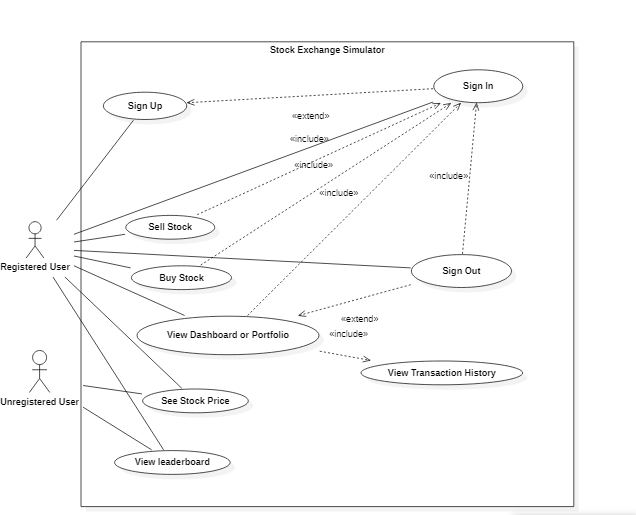
\includegraphics{usecase}
The actors are:
\begin{itemize}
\item \textbf{Unregistered Users} - Users who have not signed up yet or are signed up but do not sign in
\item \textbf{Registered Users} - Users who have signed up and are signed in.
\end{itemize}

The use cases are:
\begin{itemize}
\item \textbf{Sign Up} - Users sign up by providing their personal information on a registration page form.
\item \textbf{Sign In} - Users sign in by entering their username and password.
\item \textbf{Sign Out} - End signed in session so no one else accesses an account.
\item \textbf{See Stock Price} - View stock listings.
\item \textbf{Buy Stock} - Buy stock and add it to account.
\item \textbf{Sell Stock} - Sell stock already in account.
\item \textbf{View Dashboard or Portfolio} - Users view their stocks, their valuations and other statistics on a dashboard page.
\item \textbf{View Transaction History} - Users view their stock buying and selling history.
\item \textbf{View Leaderboard} - Users see all users along with their valuations and ranked accordingly.
\end{itemize}
	
	TO DO: Provide a use case diagram which will encapsulate the entire system and all possible actors. Do not include detailed use case descriptions (these will be needed when you will be working on the Test Plan), but make sure to include a short description of what every use-case is, who are the actors in your diagram.
	
	\chapter {Other Non-Functional Requirements}
	\section {Performance Requirements}
	\textit{If there are performance requirements for the product under various circumstances, state them here and explain their rationale, to help the developers understand the intent and make suitable design choices. Specify the timing relationships for real time systems. Make such requirements as specific as possible. You may need to state performance requirements for individual functional requirements or features. 
	TODO: Provide at least 5 different performance requirements based on the information you collected from the client. For example you can say “1. Any transaction will not take more than 10 seconds, etc…}
	\subsection{Application start-up time}
	The application should not take more than 10 seconds to load
	\subsection{Switching pages}
	The application should load any new page clicked on by the user in no more than 5 seconds
	\subsection{Authentication}
	Results of authentication (for example successful or failed sign-in or signup) should be obtained in no more than 5 seconds.
	\subsection{Stock price quote}
	Searching for a stock and getting its price from the quote page should not take more than 15 seconds
	\subsection{Buy/Sell Stocks Transactions}
	Result of buying and selling a stock should not take more than 10 seconds.
	
	
	\section {Safety and Security Requirements}
	\subsection{Safety Requirements}
	This product does not have any particular safety hazards other than the common problems associated with long periods of computer usage such as the following:
	\begin{itemize}
		\item eye strain / weakening of eyesight
		\item headaches
		\item postural issues and muscular imbalances
	\end{itemize}
	As such, it is the responsibility of the end user themself to avoid using the application for prolonged periods of time and take regular breaks.
	
	\subsection{Security Requirements}
	\begin{itemize}
		\item Users' passwords must be stored safely and not leaked in any case
		\item Every user's data must be protected from tampering by any other user
	\end{itemize}
	Security related to authentication would be satisfied easily as Google's trusted Firebase system would be used for authentication. However for database security, the developers must design the Firestore database and define its security and access rules properly.
		
	\section {Software Quality Attributes}
	\subsection{Readability}
	The developers must ensure that the code they write is clean and highly readable, for ease of future development. Bad practices must be avoided. Clear and consise comments should be provided.
	\subsection{Maintainability}
	Although high readability would play a part in making the code maintainable, additional efforts must be made in this regard such as modularization of code as much as possible and making each module perform small independent tasks.
	\subsection{Adaptability}
	The code must be written in such a way that it can be easily adapted to changes in syntax, functionality, etc. of Firebase and Alpha Vantage API.
	\subsection{Reuseability}
	The modules of the program must be reusable to make it easy to extend and enhance this application in future versions.
	\subsection{Robustness}
	The main reason for crashes in the application could be change in syntax and functionality of Firebase or Alpha Vantage API. Developers must keep this fact in mind and expect such changes. User's data must not be affected in such situations and the program must not give any output that is not easy to understand for a common user.
	\subsection{Usability}
	The application's functions and user interface must be designed while keeping in mind that most of the end users would be common people who may not have much technical expertise and just want to learn stock trading. As such the application must be very simple, easy to use, and intuitive.
		
	\chapter {Other Requirements}
	This section is Optional. Define any other requirements not covered elsewhere in the SRS. This might include database requirements, internationalization requirements, legal requirements, reuse objectives for the project, and so on. Add any new sections that are pertinent to the project.
		
	\chapter {Appendix A - Data Dictionary}
	Data dictionary is used to track all the different variables, states and functional requirements that you described in your document. Make sure to include the complete list of all constants, state variables (and their possible states), inputs and outputs in a table. In the table, include the description of these items as well as all related operations and requirements.
		
	\end{document}
